
\documentclass[12pt,twoside]{article}

\usepackage{styles/weiiszablon}
\usepackage{styles/listings-rust}
% uzywane do wyrownywania obrazkow (FloatBarrier)
\usepackage{placeins}

\author{Michał Majda}

% np. EF-123456, EN-654321, ...
\studentID{EF-157100}
\title{Proceduralne generowanie map \\ z wykorzystaniem w grze typu roguelike }
\titleEN{Temat pracy po angielsku}
\newcommand{\rodzajPracyNo}{1}
\supervisor{dr hab. inż. Maciej Kusy, prof. PRz }
\supervisorEN{(academic degree) Imię i nazwisko opiekuna}

\abstract{Treść streszczenia po polsku}
\abstractEN{Treść streszczenia po angielsku}

\begin{document}

% strona tytułowa
\maketitle

\blankpage
\tableofcontents
\clearpage
\blankpage


% \section*{Wykaz symboli, oznaczeń i skrótów (opcjonalny)}
% \addcontentsline{toc}{section}{Wykaz symboli, oznaczeń i skrótów (opcjonalny)}%
%
% 1 $\div$ 2 stron wykaz ważniejszych symboli i oznaczeń (jeśli jest potrzebny).
% \clearpage

\section*{Wstęp}
Roguelike to gatunek gier komputerowych posiadający elementy gier RPG TODO[ksiazka o rpg], bazujący na dużej losowości rozgrywki \cite{bookroguelike}. Losowość w tych grach W głównej mierze opiera się na losowym rozmieszczeniu przeciwników i przedmiotów oraz losowo generowanych mapach. Inna wążną cechą gier Roguelike jest permadeath -- śmierć gracza oznacza konieczność gry od początku. Klasyczne roguelike-i z racji trudnej rozgrywki nie były popularne, ale w ostatnich latach coraz popularniejsze są gry inspirujące się tym gatunek biorąc z niego tylko wybrane elementy. Z powodu standardowej dla roguelike-ów słabej jakościowo grafiki, oraz map tworzonych proceduralnie to znaczy według algorytmów zamiast ręcznie, gry te są stosunkowo proste w produkcji i nawet współcześnie możliwe do zrealizowania przez jedną lub dwie osoby. Nowsze gry posiadające elementy roguelike najczęściej rezygnują z stanardowego dla starszych tytułów systemu turowego oraz ruchu po kwadratowej siatce na rzecz gry w czasie rzeczywistym i swobodnego ruchu. Czyni to nowych przedstawicieli gatunku roguelike bardziej przystępnymi co przekłada się na wzrost popularności TODO[zrodlo pupularnosc roguelike].

Gatunek ten zapoczątkowany został przez grę Rogue w 1980 roku TODO[ksiazka o rogue], od tej gry wzięła się też nazwa gatunku roguelike - Rogue podobne. Rogue gracz eksploruje podziemia walcząc z przeciwnikami oraz zdobywając coraz lepszy ekwipunek, celem ukończenia gry jest zdobycie amuletu Yendoru znajdującego się w najniższym poziomie. Grafika oparka jest o znaki tekstowe ASCII  TODO[ksiazka o ascii], rozgrywka dzieje się w systemie turowym na kwadratowej siatce.

Mimo iż gatunek roguelike rozwinął się znacznie to wciąż powstają gry wierne klasycznym założeniom gatunku. Przykładem takiej gry jest Caves of Qud z 2015 roku TODO[zrodlo coq]. Gra ta posiada wszystkie cechy klasycznego roguelike-a - turowa rozgrywka, permadeath oraz ruch po kwadratowej siatce, jednak klasyczną grafikę tekstową zastąpiono prostą grafiką typu pixel art TODO[zrodlo pixel art] w formacie 16x24 piksele na jeden kwadrat na mapie.

Jednym z najbardziej popularnych przykładów nowoczesnych roguelike-ów jest gra The Binding of Isaac z roku 2011 TODO[zrodlo isaac]. Z gatunku roguelike gra ta zaczerpnęła losowe generowanie map, przedmiotów i przeciwników oraz permadeath. W The Binding of Isaac rozgrywka dzieje się w czasie rzeczywistym a ruch gracza nie jest ograniczony do siatki, dzięki temu gra jest bardziej zręcznościowa i łatwiejsza.\\

Głównym celem pracy jest stworzenie gry z gatunku roguelike z proceduralnei generowanymi mapami, oraz omówienie użytych metod generacji map. \\

Struktura pracy jest następująca: W rozdziale pierwszym dokonano szczegółowej charakterystyki porównawczej innych gier z gatunku roguelike: Rogue, Caves of Qud, The Binding of Isaac. Rozdział drugi opisuje grę roguelike stworzoną na potrzeby niniejszej pracy, w rodziale trzecim zaprezentowano proces tworzenia tej gry oraz omówienie metod proceduralnego generowania map.

\clearpage

%%%%%%%%%%%%%%%%%%%%%%%%%%%%%%%%%%%%%%%%%%%%%%%%%%%%%%%%%%%
% z szablonu
\iffalse
Do 20\% objętości pracy. W zależności od charakteru pracy ten rozdział powinien zawierać:
\begin{enumerate}[label=\alph*), leftmargin=1.25cm]
	\item opis tematyki zagadnienia -- aktualny stan zagadnienia,
	\item metody i rozwiązania,
	\item dyskusja i krytyczna ocena stanu aktualnego,
	\item podsumowanie stanu wiedzy, techniki literaturowe itp.
\end{enumerate}


\subsection{Formatowanie rozdziałów i podrozdziałów}
Rozdziały zaczynają się u góry nowej strony (parzystej lub nieparzystej). Podrozdziały i zakresy mogą zaczynać się w dowolnym miejscu strony. Przy końcu pracy zamieszcza się podsumowanie i wnioski. Ostatni akapit podsumowania musi zawierać wyszczególnienie własnej pracy Autora i zaczynać się od sformułowania: „Autor za własny wkład pracy uważa:”. W tym miejscu kończy się numeracja rozdziałów.

Ewentualne listingi programów, instrukcje obsługi stanowisk lub inne tego rodzaju materiały zaleca się zamieścić w formie dodatków. Kolejno zamieszcza się: wykaz literatury, spis rysunków/tabel oraz streszczenie (zgodne ze „Wzorem streszczenia”). Wykaz literatury rozpoczyna od strony nieparzystej.

Opisując własne dokonania, stosuje się formę bezosobową w czasie przeszłym np. celem pracy było zaprojektowanie\ldots, zakres pracy obejmował wyznaczenie\ldots, w~ramach pracy wykonano model\ldots itp.

\fi
%%%%%%%%%%%%%%%%%%%%%%%%%%%%%%%%%%%%%%%%%%%%%%%%%%%%%%%%%%%%%%%%%%%%

\section{Charakterystyka porównawcza gier roguelike}

W niniejszym rodziale szczegółowo omówiono przykłowe gry z gatunku roguelike. Omówione gry to 1: Rogue, 2: Caves of Qud, 3: The Binding of Isaac. Gatunek roguelike od swoich początków nie jest mocno popularnym gatunkiem z powodu trudnej rozgrywki, skomplikowanego sterowania oraz prymitywnej oprawy graficznej. Powstały jednak popularne gry, które zaczerpują z gatunku tylko niektóre elementy, co w niektórych przypadka oznacza płynną, prostszą rozgrywkę z elementami roguelike.

\subsection{Rogue}

Rogue: Exploring the Dungeons of Doom to zaprogramowana w 1980 roku przez Michael-a Toy i Glenn-a Wichman w języku C gra, która zapoczątkowała gatunek Roguelike. Gracz wciela się w postać podróżującą w głąb podziemi osadzonych w fantastycznym, średniowiecznym świecie, w celu odnaleznia amuletu Yendoru. Rogue nie posiada wyboru ani konfiguracji postacji, dlatego każdy gracz rozpoczyna grę tą samą postacią. W trakcie rozgrywki napotkać można wielu przeciwników, a w walce z nimi pomagają znajdowane na poziomach przedmioty i ekwpiunek. Podczas eksploracji glebszych poziomów podziemi gracz napotyka coraz trudniejszych przeciwników, lecz także przedmioty, które znajduje są coraz lepsze. Gra Rogue oparta jest o system turowy, przeciwnicy mogą wykonać ruch dopiero po ruchu gracza. W wyniku tego gra pozwala na dowolnie długie przemyślenie każdego ruchu i taktyczne podejście do walki. Każda mapa przedstawiona jest za pomocą siatki kwadratów, w wyniku czego ruch gracza ograniczony jest do 8 kierunków: góra, dół, lewo, prawo i ukosy. 

Z racji ograniczeń sprzętowych w czasach wydania gry Rogue za reprezentację graficzną odpowiadają litery i znaki ASCII w terminalu. Na rysunku \ref{Rogue:scr1} przedstawiono fragment rozgrywki w grze Rogue. Pomarańczowymi liniami oznaczone są ściany pokojów, zielonymi kropkami podłogi, na szaro oznaczono korytarze. Żólta twarz reprezentuje postać gracza przeciwnicy są oznaczani literami jak hobogoblin oznaczony białą literą 'H' na rysunku.

\FloatBarrier
\begin{figure}[h]
	\centering
	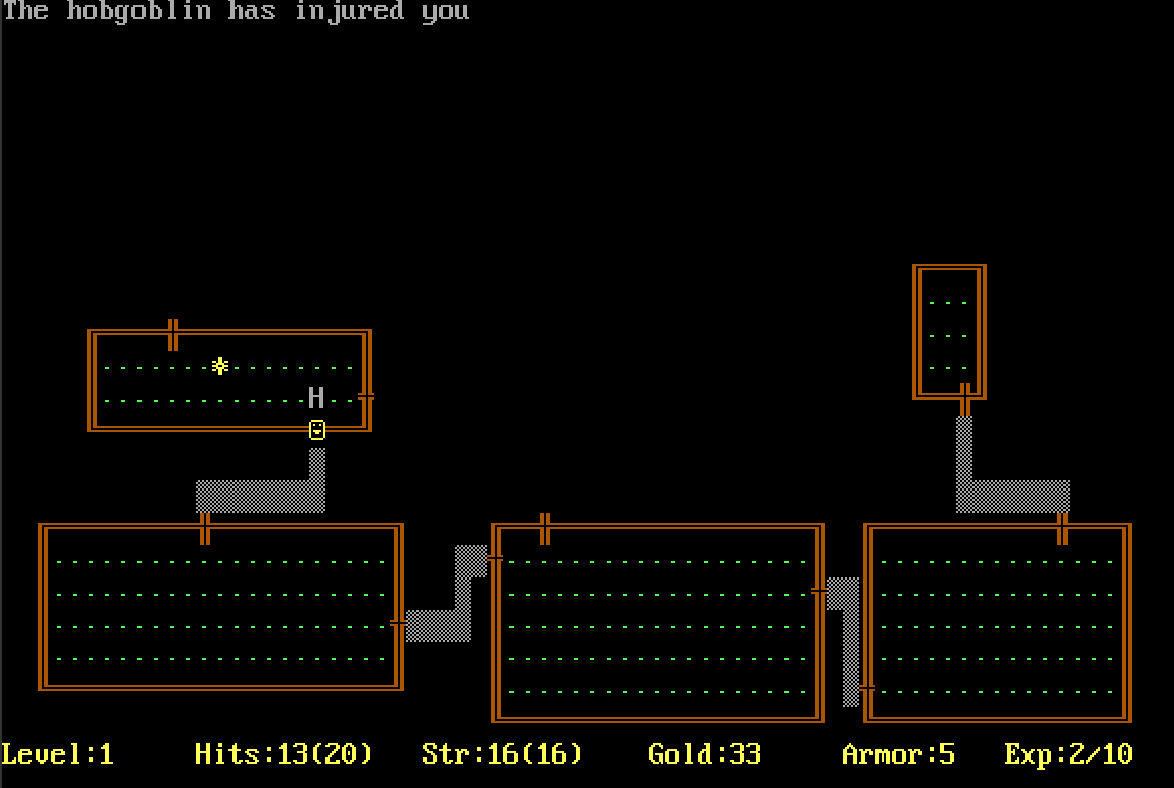
\includegraphics[width=12cm]{images/rogue/scr1.png}
	\caption{Widok główny gry Rogue}
	\label{Rogue:scr1}
\end{figure}
\FloatBarrier

Do sterowania w Rogue używana jest tylko klawiatura, do poruszania przeznaczone są klawisze klawiatury numerycznej a do wykonywania akcji litery -- na przykład klawisz 'I' służy do wyswietlenia ekwipunku. Aby zaatakować gracz musi poruszyć się w stronę przeciwnika będąc tuż przy nim. Wyświetlanie ekwipunku w grze Rogue pokazano na rysunku \ref{Rogue:scr2}, manipulowanie przedmiotami w plecaku nie odbywa się w tym oknie, ale w głownym widoku gry za pomocą odpowienich klawiszy i podania litery odpowiadającej danemu przedmiotowi w ekwipunku. Na przykład aby wyrzucić przedmiot 'a +1, +1 mace` znajdujący się w ekwipunku na rysunku \ref{Rogue:scr2} trzeba wcisnąć klaiwsz 'd' odpowiadający za wyrzucanie przedmiotów i literę 'c' przypisaną obecnie do tego przedmiotu, a w celu zjedzenia 'some food' klaiwsz 'e' odpowiadający za akcję jedzenia i literę 'a'. 

\FloatBarrier
\begin{figure}[h]
	\centering
	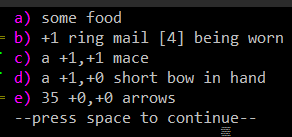
\includegraphics[width=8cm]{images/rogue/scr2.png}
	\caption{Ekran ekwipunku w Rogue}
	\label{Rogue:scr2}
\end{figure}
\FloatBarrier

Rogue zawiera proste proceduralnie generowane mapy, przykładowe dwie mapy pokazano na rysunku: \ref{Rogue:scr3}. Każda mapa zawiera pokoje w układzie siatki 3x3, co szczególnie widać na mapie po prawej na rysunku \ref{Rogue:scr3}, maksymalna liczba pokojów to dziewięć, ale może być ich mniej. Pokoje są połączone ze sobą korytarzami a niektóre przejścia mogą być ukryte przed graczem, co wymusza częste korzystanie z komendy przeszukiwania dostępnej pod klawiszem 'S'. Pokoje i korytarze mogą zawierać ukryte pułapki, które można wykryć używając komendy szukania. Jedyną zmianą w głebszych poziomach są małe labirynty umiejszczone czasami w miejsce niektórych pokojów.

\FloatBarrier
\begin{figure}[h]
	\centering
	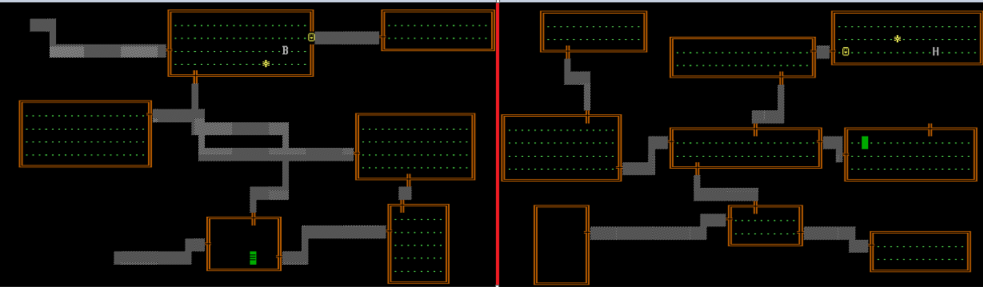
\includegraphics[width=16cm]{images/rogue/scr3.png}
	\caption{Przykładowe mapy w grze Rogue}
	\label{Rogue:scr3}
\end{figure}
\FloatBarrier

Z racji sporego wieku gry Rogue ciężko jest określić jej popularność, jednak z pewnością można stwierdzić, że jest to kluczowa dla gatunku roguelike gra, która stworzyła podwaliny jego głównych cech. Świadczy o tym między innymi sama nazwa gatunku roguelike, która oznacza "podobne do Rogue".



\subsection{Caves of Qud}
Caves of Qud to współczesny przykład rozwoju klasycznej formuły roguelike-ów. Gra tworzona jest w silniku Unity przez studio Freehold Games, wydana została w 2015 roku, lecz rozwijana jest do dzisiaj (stan na luty 2022 roku). Gra posiada wszystkie cechy klasycznego roguelike-a: działa w systemie turowym, posiada permadeath, mapa gry oparta jest o siatkę kwadratów, lecz dodaje też sporo nowoczesnych rozwiązań i znaczne rozwinięcie wielu mechanik gry. Caves of Qud osadzone jest w post apokaliptycznym fantastycznym świecie w którym zaawansowana technologia miesza się z fantastycznymi rasami oraz magią.

Jednym z głównych wyróżników Caves of Qud na tle innych gier tego typu jest bardzo mocno rozwinięty system proceduralnie generowanych map. Gra posiada otwarty świat o statycznie umiejscowionych obszarach takich jak góry, dżungle i pustynie a także miastach, na rysunku \ref{CoQ:scr1} przedstawiono przykładowe mapy wygenerowane w tej grze. Pomimo statycznego ustawienia konkretnych obszarów w grze sam wygląd danych obszarów i miejsc jest proceduralnie generowany, a także na wielu mapach mogą zostać dodane obiekty takie jak ruiny, obozowiska i tym podobne. Główną i najbardziej interesującą metodą uzywaną w tej grze jest generowanie map oparte o Wave Function Collapse (Załamanie funkcji falowej) \cite{coq_wfc}. Metoda ta pozwala na generowanie dowolnych map opartych o mały wzorzec.

\FloatBarrier
\begin{figure}[h]
	\centering
	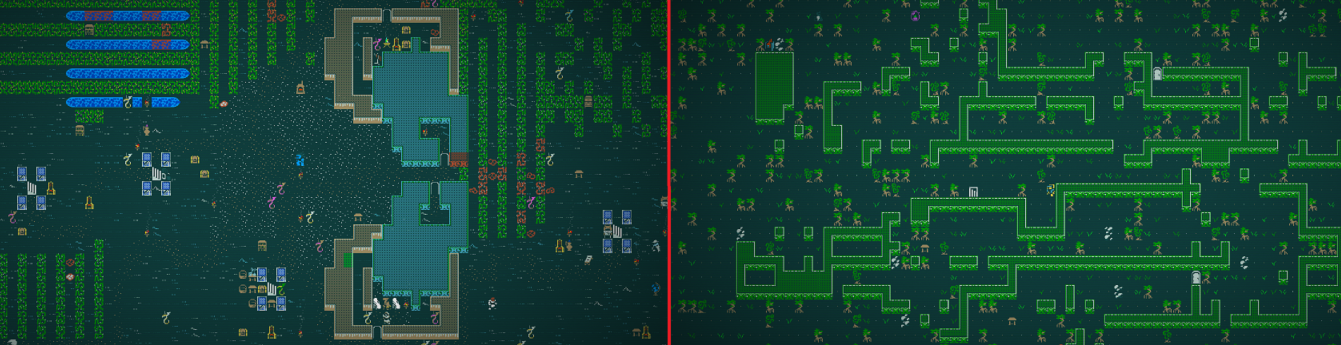
\includegraphics[width=16cm]{images/caves_of_qud/scr1.png}
	\caption{Przykładowe mapy w grze Caves of Qud. Po lewej wioska, po prawej dżungla z ruinami}
	\label{CoQ:scr1}
\end{figure}
\FloatBarrier

Podobnie jak w grze Rogue tutaj również do poruszania się używana jest klawiatura numeryczne i klawisze liter do dostępu do ekwipunku, listy zadań i tym podobne, lecz Caves of Qud umożliwia też granie wyłącznie za pomocą myszki. Gra oferuje bardziej przejrzystę grafikę typu pixel art co przedstawiono na rysunku \ref{CoQ:scr3}.

\FloatBarrier
\begin{figure}[h]
	\centering
	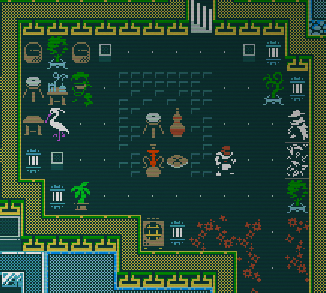
\includegraphics[width=8cm]{images/caves_of_qud/scr3.png}
	\caption{Zrzut ekranu z gry Caves of Qud}
	\label{CoQ:scr3}
\end{figure}
\FloatBarrier

Caves of Qud znacznie rozwinęło też interfejs użytkownika, co znacząco wpływa na ułatwienie rozgrywki. Interfejs jest tu przejrzysty i prosty, dzięki czemu zmiana ekwipunku oraz używanie przedmiotów jest dużo łatwiejsze. Na rysunku \ref{CoQ:scr2} przedstawiono ekran ekwipunku.

\FloatBarrier
\begin{figure}[h]
	\centering
	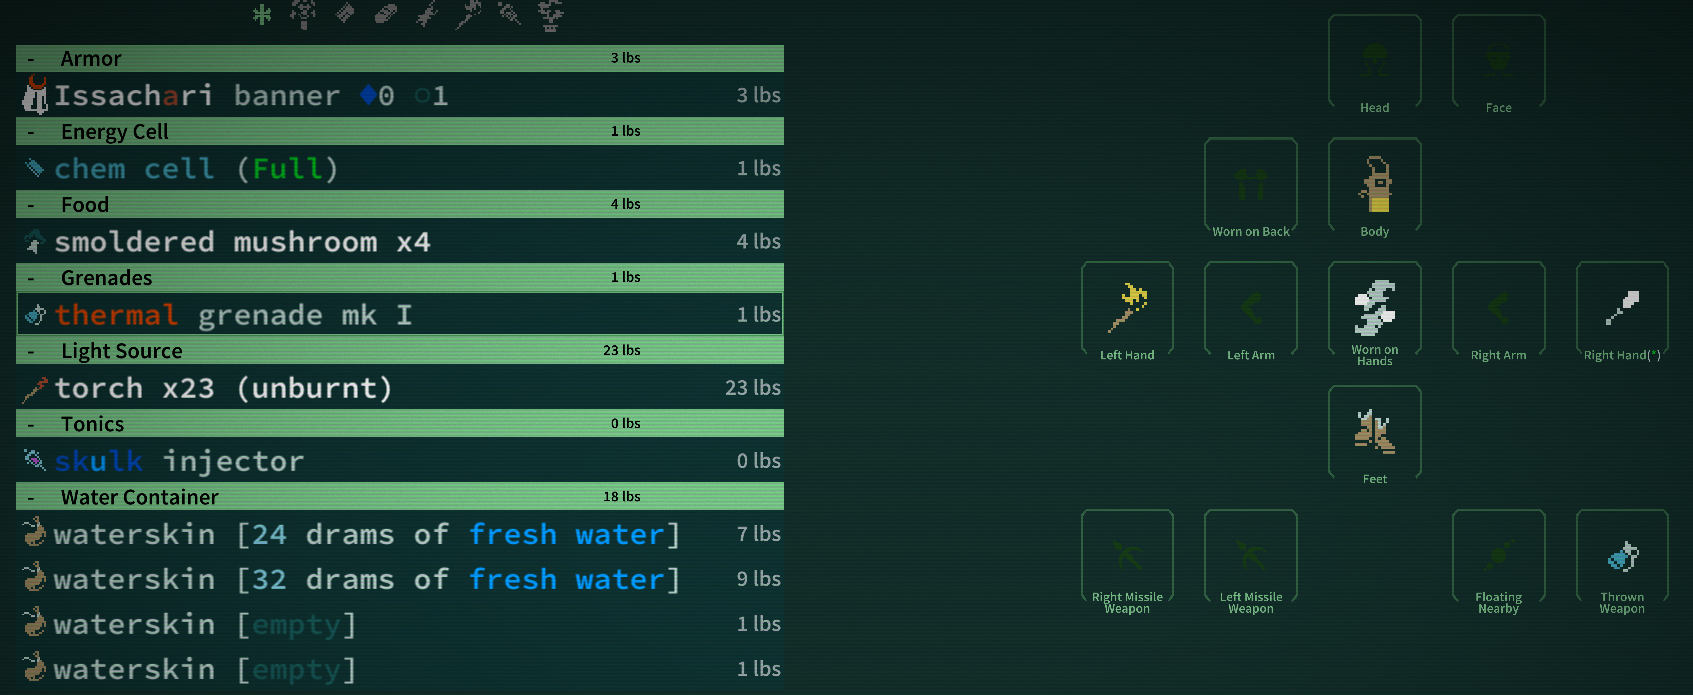
\includegraphics[width=14cm]{images/caves_of_qud/scr2.png}
	\caption{Ekran ekwipunku w Caves of Qud}
	\label{CoQ:scr2}
\end{figure}
\FloatBarrier

Interesującym rozwiązaniem w Caves of Qud jest system handlowy. W grze istnieje system głodu i pragnienia, gracz więc w celu uniknięcia śmierci z głodu lub odwodnienia musi nosić ze sobą zapasy wody i pożywienia, które mają swoją wagę, więc można ich posiadać ograniczoną ilość. Walutą w tej grze jest woda pitna, która jest bardzo rzadko spotykana w postaci źródeł, zdecydowana większość wody w zbiornikach naturalnych jest niezdatna do picia. Z tego powodu gracz zbiera wodę nie tylko dla zaspokojenia pragnienia, ale również w celu handlu z spotykanymi między innymi w wioskach handlarzami. Postać gracza ma ograniczony udźwig, więc często handel sprowadza się do handlu wymiennego, ponieważ trudno jest nosić ze sobą duże kwoty w postaci wody.

Gra Caves of Qud znacznie rozwija aspekt RPG -- odgrywania postaci. W trakcie wyboru postaci najpierw wybiera się typ postaci - mutant mający dostęp do wielu fizycznych lub mentalnych mutacji, które zapewniają dodatkowe zdolności, bonusy lub nawet dodatkowe kończyny lub True Kin będący niezmutowanym człowiekiem, który ma dostęp do cybernetycznych implantów dających różnorodne bonusy i umiejętności. Poza typem wybiera się też pochodzenie postaci, które określa początkowy ekwipunek oraz bonusy do atrybutów. W trakcie gry gracz może dowolnie rozwijać -- zwiększając wartości atrybutów takich jak siła, zręczność, siła woli i tym podobne oraz przez uczenie się nowych umiejętności jak specjizacja w posługiwaniu się konkretnym typem broni lub lepszego unikania ataków. Dzięki dostępowi do dużej ilości różnorodnych mutacji lub implantów, zależnie od typu postaci, gracz dodatkowo może kreować swoją postać na wiele sposobów.

W Caves of Qud proceduralne generowanie używane jest nie tylko do generowania map. W grze można znaleźć duże ilości proceduralnie tworzonych książek, z których część dotyczy także samej fabuły gry \cite{coq_history}. Oznacza to, że poza niektórymi stałymi we wszystkich rozgrywkach aspektami historii również część fabuły będzie inna w każdej nowej rozgrywce.

W odróżnieniu od większości gier tego typu Caves of Qud posiada mocno rozwiniętą historię i rozbudowane główne zadania fabularne. Poza główną linią zadań gra oferuje też sporo losowych zadań, które jednak są dosyć proste i najczęściej sprowadzają się do zdobycia konkretnego przedmiotu lub znalezienia jakiegoś miejsca. Główne zadania są różnorodne, często polegają na odwiedzaniu fabularnych, rozbudowanych lokacji, obronie pewnego miasta przed atakiem lub nawet rozwiązywania zagadek.

Biorąc pod uwagę fakt, że klasyczne gry typu roquelike posiadające dość wysoki poziom trudności rozgrywki, wciąż uznawane są za dość niszowy gatunek. Poszczególne gry zyskują jednak relatywnie dużą popularność, czego przykladem jest Caves Qud, które w serwisie Steam posiada 4356 z czego 95\% jest pozytywnych (stan na luty 2022) \cite{coq_steam}.



\subsection{The Binding of Isaac}

Gra The Binding of Isaac została stworzona w roku 2011 przez Edmund-a McMillen i Florian-a Himsl, a następnie jako remake The Binding of Isaac: Rebirth w roku 2014. W niniejszej pracy skupiono się na omówieniu The Binding of Isaac: Rebirth, gdyż jest to nowsza i bardziej popularna odsłona. Gra ta jest przykładem wzorowania się na roguelike-ach, ale odejściu od części klasycznych założen. Z gatunku zaczerpnięto losowo generowane mapy, losowo rozmieszczane przedmioty i przeciwników, oraz konieczność grania od początku w przypadku śmierci głównej postaci. Rozgrywka w The Binding Isaac dzieje się w czasie rzeczywistym, a ruch postaci nie jest ograniczony do siatki kwadratów. Z tego powodu gra jest bardzo dynamiczna, a walka zręcznościowa.

The Binding of Isaac odeszło od podziału mapy na kwadratową siątke, ale wciąż korzysta z względnie prostej grafiki typu pixel art, co przedstawiono na rysunku: \ref{tboi:scr1}.

\FloatBarrier
\begin{figure}[h]
	\centering
	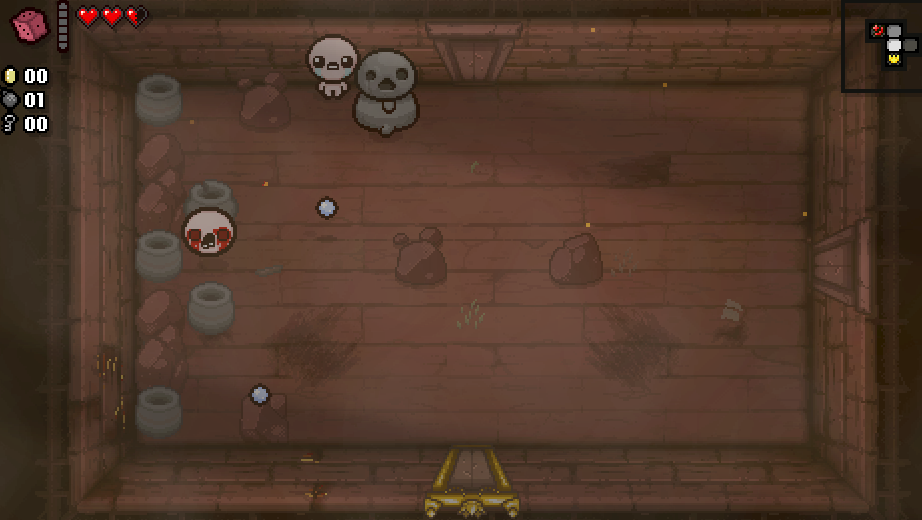
\includegraphics[width=10cm]{images/tboi/scr1.png}
	\caption{Przykład rozgrywki w The Binding of Isaac: Rebirth}
	\label{tboi:scr1}
\end{figure}
\FloatBarrier

Gracz wciela się początkowo w postać Isaac, ale w trakcie rozgrywki może odblokować wiele nowych postaci, które różnią się początkowymi statyskimi takimi jak zdrowie i siła ataku oraz posiadanymi przedmiotami. Gra nie posiada typowego ekwipunku takiego jak zbroje i bronie, zamiast tego w grze zbiera się nieograniczoną ilość przeróżnych przedmiotów, które zapewniają pasywne bonusy. Bonusy te wzmacniają postać na wiele różnych sposobów, od podstawowych zwiększających zdrowie lub atak po takie, które zmieniają łzy, którymi strzela gracz na zupełnie inną postać. Jednym z głównym aututów The Binding of Isaac są możliwe kombinacje przedmiotów, przykładowo jeśli gracz zdobędzie przedmiot, dzięki któremu pociski postaci będą się same nakierowywały na przeciwników, a następnie przedmiot, który zamienia pociski na laser, to ten laser będzie zaginany tak, aby zawsze trafiać przeciwników bez konieczności celowania, co pokazano na rysunku \ref{tboi:scr2}.


\FloatBarrier
\begin{figure}[h]
	\centering
	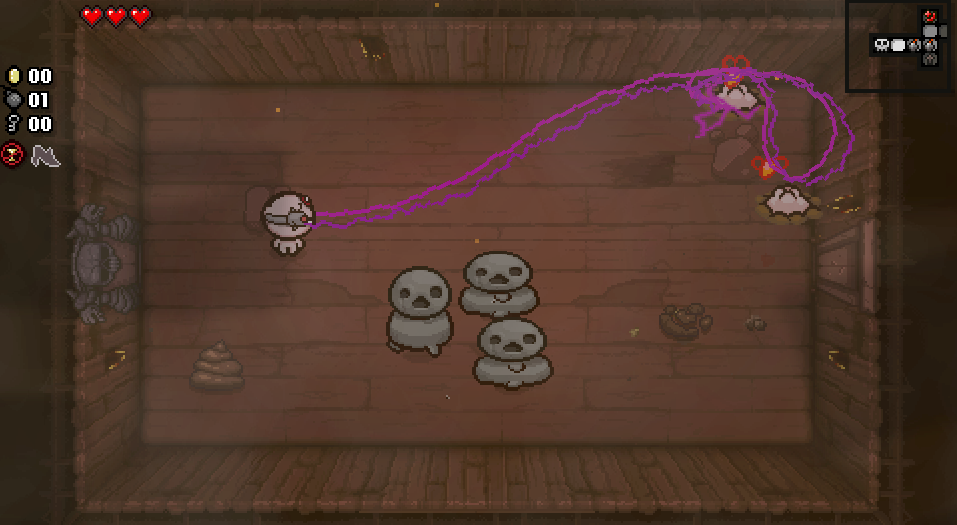
\includegraphics[width=10cm]{images/tboi/scr2.png}
	\caption{Przykład kombinacji przedmiotów w The Binding of Isaac: Rebirth}
	\label{tboi:scr2}
\end{figure}
\FloatBarrier

W grze The Binding of Isaac za sterowanie postacią odpowiadają klawisze 'W', 'A', 'S', 'D' , a za strzelanie klawisze strzałek, do używania przedmiotów jest też używana spacja i klawisz 'Q'. Proste sterowanie jest kolejnym powodem przystępności tej gry.
 W porównaniu do innych gier roguelike losowo generowane mapy w The Binding of Isaac są znacznie prostsze. Gra składa się z wielu poziomów podzielonych na pokoje, każdy z poziomów zakończony jest walką z silnym przeciwnikiem -- bossem. Pokoje są wybierane losowo z puli pokojów przygotowanych przez twórców, a ich rozkład i połączenia są losowo generowane. Na rysunku \ref{tboi:scr3} przedstawiono przykładowy układ poziomów. Z każdym kolejnym poziomem ilość pokojów jest coraz większa, ale jakość napotykanych przedmiotów nie wzrasta. Napotykane przedmioty są kompletnie losowe, dlatego czasem już nawet po pierwszym poziomie postać gracza może posiadać kilka najsilniejszych przedmiotów. 

\FloatBarrier
\begin{figure}[h]
	\centering
	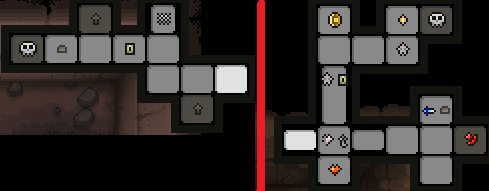
\includegraphics[width=12cm]{images/tboi/scr3.png}
	\caption{Przykład układ poziomów w The Binding of Isaac: Rebirth}
	\label{tboi:scr3}
\end{figure}
\FloatBarrier

Jedną z cech gier gatunku roguelike, które implementuje The Binding of Isaac jest permadeath. W porównaniu jednak do innych do tytułów, na których ukończenie trzeba często poświęcić parę godzi, The Binding of Isaac sprawnemu graczowi zajmie około godzinę na ukończenie, w wyniku czego rozpoczynanie rozgrywki od początku nie jest tak dotkliwe, i zachęca do częstego powtórnego przechodzenia gry.


The Binging of Isaac: Rebirth jest jedną z najbardziej popularnych gier z gatunku roguelike, na serwisie Steam posiada 166244 opini, w tym 97\% pozytwnych (stan na luty 2022) \cite{tboi_steam}. Dowodzi to, że przeciętny gracz woli dynamiczną, rozgrywaną w czasie rzeczywistym rozgrywkę od wolnej, taktycznej rozgrywki turowej.

\clearpage	


\section{Szczegółowy opis gry}

W ninejszym rozdziale przedstawiono wszystkie elementy i możliwości gry z gatunku roguelike stworzonej na potrzeby niniejszej pracy.



































Ponad 50\% objętości pracy -- część autorska:
\begin{enumerate}[label=\alph*), leftmargin=1.25cm] 
	\item założenia – dane,
	\item opis zastosowanej metody rozwiązania lub analizy,
	\item opis proponowanego rozwiązania, wyniki analizy teoretycznej, obliczenia, projekt konstrukcyjny, procesowy, technologiczny,
	\item wyniki badań analitycznych, symulacyjnych lub eksperymentalnych itp.
\end{enumerate}

Przy stosowaniu podziału na rozdziały i podrozdziały zaleca się unikać podziału więcej niż trzystopniowego. Podział tekstu, szczególnie na rozdziały główne, wynikać powinien z zakresu i charakterystyki realizowanej pracy.

\subsection{Formatowanie tekstu. Należy pamiętać, że na końcu tytułu rozdziału, podrozdziału i zakresu nie umieszcza się kropki}

\subsubsection{Marginesy i akapity}

Marginesy deklaruje się jako „lustrzane” i ustawia na 2 cm, na oprawę 1,5 cm. 
Nagłówek i stopka 1,25 cm. Tekst podstawowy akapitu: czcionka szeryfowa, styl Times (Times New Roman, Liberation Serif itp.), rozmiar 12 punktów, interlinia 1,5 wiersza. Akapit wyjustowany, wcięcie pierwszego wiersza 1,25 cm. 

Na końcu każdego akapitu, którego tekst zaczerpnięto z literatury, musi znajdować się odnośnik do właściwej pozycji w wykazie literatury. W pracy nie stosuje się
odnośników w formie przypisów. Liczby w nawiasie kwadratowym oznaczają kolejny numer pozycji w wykazie, np. [1] lub [1, 4, 7] lub [1, 6-8] itp.

Cytaty (dosłowne przytoczenie obcego tekstu w pracy) pisze się czcionką pochyłą (kursywą) i ujmuje w cudzysłów. Przykład: „\textit{Współpracując z jednostkami gospodarczymi działającymi w kraju, kształci wysokokwalifikowaną kadrę inżynierów}”.

Fragmenty kodów programów pisze się czcionką o stałej szerokości, styl \footnotesize {\texttt{Courier}}
\normalsize{(Courier New, Liberation Mono itp.) o rozmiarze 10 punktów.}


\subsubsection{Zalecenia co do sposobu pisania jednostek i symboli wielkości fizycznych}

Poniższy podrozdział opracowano na podstawie \cite{Pawluk2001}. W trakcie pisania pracy należy zwracać uwagę na sposób oznaczania jednostek i symboli wielkości fizycznych. Przy zapisywaniu jednostek i symboli wielkości fizycznych można wyróżnić zapis w~postaci kursywy (pismo pochyłe) oraz antykwy (pismo proste). 

\begin{enumerate}[label=\arabic*), leftmargin=1.25cm]
\item Kursywę należy stosować w następujących przypadkach:

\begin{itemize}[label=-,labelsep=0.4cm,leftmargin=0.6cm] %[leftmargin=0.65cm]
\item symboli wielkości fizycznych niezależnie od tego czy jest to litera alfabetu greckiego (np. przenikalność magnetyczna $\mu$) czy też łacińskiego (np. rezystancja $R$). Należy przestrzegać tej zasady niezależnie od miejsca, w którym pojawia się symbol tj. tekst, wzory matematyczne, rysunki, tabele,

\item ogólny symbol zapisu funkcji czyli np. $f$, a nie f. Nie dotyczy to jednak zapisu konkretnych funkcji np. $\cos \omega t$ a nie $cos \omega t$,

\item macierze, wektory, których elementami są wielkości fizyczne należy zapisywać dodatkowo czcionką półgrubą (bold) np. 
$\bm{R} = \left[ 
\begin{array}{cc}
R_{11} & R_{12} \\
R_{21} & R_{22} 
\end{array} 
\right]$,
$\bm{U} = \left[ 
\begin{array}{c}
U_{1} \\
U_{2} 
\end{array} 
\right]$,

\item wskaźnik dolny, górny, prawo- i lewostronny, ale tylko gdy odnosi się do konkretnej wielkości fizycznej, czyli np. składowa $x$-owa indukcji magnetycznej $B_x$, a nie $B_{\mathrm{x}}$,

\item wskaźniki górne i dolne oznaczające dowolną liczbę np. $R_j$, $I^k$, ale nie $R_\mathit{1}$, $I^\mathit{2}$.

\end{itemize}

\item Antykwę należy stosować w następujących sytuacjach:

\begin{itemize}[label=-,labelsep=0.4cm,leftmargin=0.6cm]
\item wszystkie cyfry,

\item symbole konkretnych funkcji np. $\mathrm{tg\ } \omega t$, a nie $tg \omega t$,

\item operatory operacji matematycznych np. pochodne zwyczajne $\frac{\mathrm{d} x}{\mathrm{d} t}$, a nie $\frac{d x}{d t}$,

\item symbole liczb o konkretnej wartości np. przenikalność elektryczna próżni $\varepsilon_0 = 8,8542 \cdot 10^{-12}$ $\mathrm{F} \cdot \mathrm{m}^{-1}$, a nie $\varepsilon_0 = 8,8542 \cdot 10^{-12}$ $\mathrm{F} \cdot \mathrm{m}^{-1}$,

\item indeksy, jeżeli odnoszą się do: obiektów (fizycznych, geometrycznych), czyli, np. natężenie pola elektrycznego w punkcie A to $E_\mathrm{A}$, a nie $E_A$, zjawisk lub stanów fizycznych, np. moment obciążenia to $T_\mathrm{L}$, a nie $T_L$, do nazwisk czy też oznaczeń pierwiastków, np. straty w miedzi to $P_{\mathrm{Cu}}$ a nie $P_{Cu}$, do charakteru wielkości symbolizowanej przez literę źródłową, np. wartość maksymalna siły to $F_\mathrm{max}$, a nie $F_{max}$, oznaczeń jednostek miary np. $\mathrm{M}\Omega$, a nie $M \mathit{\Omega}$.

\end{itemize}

\item W przypadku jednostek miar (które zawsze należy pisać antykwą) zapisując konkretną wartość liczbą należy podać jej wartość i jednostkę z zachowaniem następujących zasad:

\begin{itemize}[label=-,labelsep=0.4cm,leftmargin=0.6cm]
\item zapisując wartość liczbową wielkości fizycznej po spacji należy podać jej jednostkę, ale nie nazwę jednostki np. $10 \mathrm{A}$, ale nie $10$ amper czy też $10$ amperów,

\item zapisując wartość liczbową słownie należy w tej konwencji podać też jednostkę np. dziesięć omów, ale nie dziesięć $\Omega$

\item do oznaczeń jednostek nie wolno dopisywać indeksów, np. moc wyjściowa silnika wynosi $P=100$ $\mathrm{kW}_\mathrm{out}$. W takim przypadku należy zapisać $P_\mathrm{out}=100$ $\mathrm{kW}$,

\item jednostek nie należy umieszczać w nawiasach kwadratowych, np. $I=1$ $\mathrm{[A]}$. Odstępstwem od tej zasady mogą być tabele, nagłówki kolumn, opisy osi na wykresach oraz w sporadycznych sytuacjach we wzorach matematycznych (ale tylko wówczas, gdy zależność matematyczna nie wskazuje w~jakiej jednostce wystąpi wartość liczbowa). Przykłady odstępstw zamieszczono w~podrozdziale \ref{Subsec:Rysunki-i-tabele}.   

\end{itemize}

\item W trakcie zapisu symboli wielkości matematycznych można stosować również szereg znaków diakrytycznych, jak również należy przestrzegać następujących zaleceń:

\begin{itemize}[label=-,labelsep=0.4cm,leftmargin=0.6cm]
\item wartości chwilowe podstawowych wielkości fizycznych używanych np. w elektrotechnice należy zapisać małymi literami, np. $u$, $i$, lub stosować zapis np. $u(t)$, lub stosować indeks ,,$t$'' przy wielkości, np. $U_t$,

\item wartości skuteczne wielkości okresowych należy zapisać dużą literą np. $U$, $I$, 

\item wartości szczytowe funkcji zmiennej, amplitudę funkcji sinusoidalnej czasu należy zapisać jako np. $U_\mathrm{m}$,

\item podkreślenie symboli reprezentujących wielkości fizyczne, których wartość liczbowa jest liczbą zespoloną, przy czym podkreślenie dotyczy tylko literki źródłowej np. $\underline{Z}_1$, a nie $\underline{Z_1}$,

\item kreska nad literą źródłową oznacza wartość średnią, np. $\overline{I}$ co jest równoważne $I_\mathrm{av}$.

\end{itemize}

\end{enumerate}




\subsubsection{Rysunki i tabele} \label{Subsec:Rysunki-i-tabele}
Tekst podstawowy w tabeli pisze się czcionką o rozmiarze 10 punktów, pojedyncza interlinia. Dane liczbowe – wyśrodkowane, dane tekstowe – wyrównane do lewej. Rysunki i tabele zamieszcza się wyśrodkowane na stronie, bez wcięcia pierwszego wiersza.

W akapicie poprzedzającym rysunek lub tabelę musi znajdować się krótki opis, czego dotyczy dany rysunek/tabela (odniesienie do rysunku/tabeli). Tytuły numeruje się zgodnie z kolejnością w danym rozdziale: numer\_rozdziału.numer\_tabeli/rysunku (np. rys. 2.1, tabela 3.5). W tytule rysunku/tabeli, zaczerpniętych z literatury, podaje się odnośnik do właściwej pozycji. Należy zadbać o to, aby opisy na rysunkach były czytelne (czcionka 8 punktów lub większa). Staraj się nie wymuszać numeracji, pozwól aby robił to za ciebie \LaTeX. Stosuj \verb!\label! do znakowania obiektów, do których być może w tekście się będziesz odwoływał (rozdziały, rysunki, tabele, wzory, listingi \ldots). Odwołuj się do nich w tekście  za pomocą funkcji \verb!\ref{NazwaObiektu}!. Pamiętaj, że \LaTeX\, korzystając z polecenia \verb|latex| nie odczytuje z plików .jpg, .png ich wielkości. Polecenie \verb|latex| generuje plik \verb|DVI|. Jeżeli chcesz go używać zgłosi stosowny błąd. Aby się go pozbyć zdefiniuj wielkość natywną pliku grafiki. Polecamy jednak używanie zamiast polecenia \verb|latex|, polecenie \verb|pdflatex|, wówczas problem nie wystąpi.\\

\begin{example}
[\ldots] co umożliwia wyznaczenie wartości napięcia. Na rys. \ref{Fig:schemat} przedstawiono schemat obwodu z równolegle dołączoną pojemnością $C_p$.
\end{example}

\begin{figure}[ht]
	\centering
	\includegraphics[width=6cm]{figures/fig1.png}
	\caption{Tytuł rysunku, rozmiar 11 pkt., pojedyncza interlinia, akapit wyśrodkowany, bez wcięcia pierwszego wiersza. Na końcu tytułu rysunku/tabeli nie stawia się kropki [8]}
\label{Fig:schemat}
\end{figure}

\begin{example}
[\ldots] Na rysunku \ref{Fig:wykres} pokazano przykładową zależność prądów pasmowych $i_\mathrm{ph}$ bezszczotkowego silnika prądu stałego z magnesami trwałymi w funkcji położenia wirnika $\theta$.
\end{example}

\begin{figure}[ht]
	\centering
	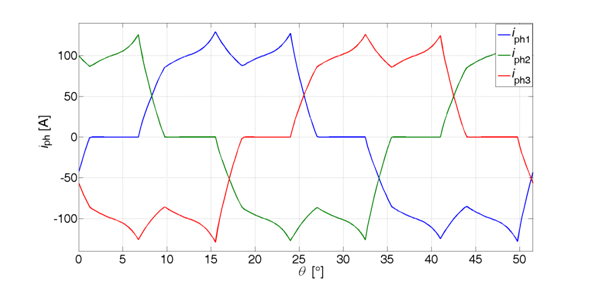
\includegraphics[width=12cm]{figures/fig2.png}
	\caption{Tytuł rysunku, rozmiar 11 pkt., pojedyncza interlinia, akapit wyśrodkowany, bez wcięcia pierwszego wiersza. Na końcu tytułu rysunku/tabeli nie stawia się kropki [8]}
\label{Fig:wykres}
\end{figure}


\begin{example}
[\ldots] oraz indukcyjności wzajemnej. W tabeli \ref{Tab:tabela} przedstawiono podstawowe parametry obwodu nieliniowego, zasilanego napięciem trójfazowym.
\end{example}

\begin{table}[ht]
\caption{Tytuł tabeli, rozmiar 11 pkt., pojedyncza interlinia, akapit wyrównany do lewej}
\centering		
	\begin{tabular}{|c|c|c|c|c|}	
		\hline
		$U$ [V] & $I$ [mA] & $R$, [k$\Omega$] & $L$ [mH] & $R/R_{20}$ \\
		\hline
		13,6 & 7,29 & 3,94 & 100 & 1,25 \\
		\hline
	\end{tabular}	
	
\label{Tab:tabela}
\end{table}	

{\subsubsection{Wzory matematyczne}}

Zmienne we wzorach pisze się czcionką pochyłą (styl edytora równań „Matematyka”) natomiast symbole, nie będące zmiennymi, czcionką prostą (styl „Tekst”).
Rozmiary czcionek: normalny 12 punktów, indeks dolny/górny 9 pkt., indeks podrzędny 7 pkt., symbol 24 pkt., podsymbol 12 pkt. Separatorem dziesiętnym w liczbach jest
przecinek, a nie kropka (dotyczy to również liczb pisanych w tekście akapitu). Poddaj się w tym zakresie \LaTeX'owi - pisz wzór, a poprawnie się utworzy.


Pod wzorem należy zamieścić objaśnienia użytych symboli (chyba, że znajdują się w wykazie na początku pracy). Wzory umieszcza się wyśrodkowane i numeruje zgodnie
z kolejnością w danym rozdziale: (numer\_rozdziału.numer\_wzoru). Numery wzorów wyrównuje się do prawego marginesu. W akapicie poprzedzającym wzór musi znajdować się krótki opis, czego dotyczy dany wzór i – jeżeli potrzeba – odwołanie do literatury.

\begin{example}
[\ldots] wyznacza się, na podstawie wyrażenia (\ref{Eq:rownanie}). W nawiasach podano rozmiary czcionek używanych we wzorach
\end{example}

\begin{equation}
A(12)={\sum}(24)m_{s(9)}N^{k_{p(7)}}
\label{Eq:rownanie}
\end{equation}
gdzie: $m_s$ -- masa próbki, $N$ -- natężenie oświetlenia, $k_p$ -- wykładnik potęgi $(k_p=1,3-2,1)$.\\
\newpage
{\subsubsection{Listingi programów}}

W pracy dyplomowej możesz umieszczać fragmenty programów. Pamiętaj, aby umieszczać krótkie, tylko najważniejsze fragmenty kodów źródłowych. Zawsze je komentuj w treści
pracy dyplomowej. Typowo w \LaTeX\ kody źródłowe umieszczane są w środowisku verbatim (\verb|\begin{verbatim}...\end{verbatim}|). Obecnie instnieje jednak bardziej nowoczesne i bardziej funkcjonalne środowisko \verb|lstlisting| (wymaga zainstalowanego w systemie pakietu \verb|listings|). Zwróć uwagę, że możesz kolorować składnię
automatycznie za pomocą parametru \verb|language|. W niniejszym dokumencie przedstawiono dwa przykłady listingów, Listing \ref{KodMatlab1} to przykład kodu źródłowego Matlaba, a poniżej Listing \ref{KodPerl1} dla Perl'a.\\
%\komentarz{


% test listingu Rust - obrazki jednak beda lepsze
\begin{lstlisting}[language=Rust,caption=Listing programu Matlab,label={KodMatlab1}]
pub fn new(x: usize, y: usize, width: usize, height: usize) -> GuiMapGenTestingManager {
	GuiMapGenTestingManager {
		x,
		y,
		width,
		height,
		selected: 0,
		bg: rltk::RGB::named(rltk::BLACK),
		title: TextCol::new(vec![("Map generators testing".to_string(),rltk::RGB::named(rltk::WHITE))]),
		options: vec![],
		options_sprites_indexes: vec![],
		show_steps: false,
		map_gen: Box::new(TestMap::new(width - 4, height - 4)),
		current_history_index: 0,
	}
}
\end{lstlisting}

\begin{lstlisting}[language=Perl,caption=Listing programu Perl,label={KodPerl1}]
  my $url ='http://pei.prz.edu.pl';
  use LWP::Simple;
  my $content = get $url;
  die "Couldn't get $url" unless defined $content;
  print $content;
  print "\n";
  print "Length " + length($content)
\end{lstlisting}

Z pewnością przeglądając źródło tego dokumentu zobaczysz, że kody źródłowe powinny mieć zdefiniowane parametry \verb|label|, aby łatwo w tekście do nich się odwoływać.
Numeracja linii jest w stylu domyślnie włączona (to przydatne, bo w treści pracy łatwo odwołać się dzięki temu do konkretnego wiersza w kodzie źródłowym), możesz je wyłączyć podając jako parametr \verb|numbers=none|. Więcej szczegółów możesz odnaleźć w sekcji \verb|\lstset| pliku arkusza styli. 
%}


\subsubsection{Numerowanie i punktowanie}

\begin{enumerate}[label=\arabic*), leftmargin=1.25cm]
	\item Pierwszy poziom (stosuje się numerowanie lub punktowanie). Formatowanie:
	akapit wyjustowany, wcięcie od lewej 0,75 cm, wysunięcie co 0,5 cm.
	\item Znakiem numerowania jest liczba (z kropką lub nawiasem).
		\begin{itemize}[label=-,labelsep=0.4cm,leftmargin=0.6cm]
			\item drugi poziom (stosuje się wyłącznie punktowanie). Formatowanie: akapit
			wyjustowany, wcięcie od lewej 1,25 cm, wysunięcie co 0,5 cm,
			\item znakiem punktowania jest łącznik lub mała litera alfabetu (z nawiasem). Nie
			zaleca się stosowania kropek, strzałek itp.,
			\item punktowane akapity rozpoczyna się minuskułą (małą literą), na końcu akapitu
			stawia się przecinek, ostatni punktowany akapit kończy się kropką.
		\end{itemize}
	\item Numerowane akapity rozpoczyna się majuskułą (wielką literą) i kończy kropką.
	\item Należy zwrócić uwagę, aby nie rozdzielać numerowania/punktowania pomiędzy
	kolejnymi stronami tekstu.
\end{enumerate}


\subsection{Wykaz literatury}

W wykazie literatury zamieszcza się wyłącznie pozycje, na które powołano się
w pracy. Kolejność numerów w wykazie – zgodna z kolejnością pojawiania się danej
pozycji w tekście.

Format akapitu: akapit wyjustowany, wysunięcie 0,75 cm. Prawidłowo opracowany
wykaz został zaprezentowany w niniejszym dokumencie w odpowiednim rozdziale, oznaczonym jako „Literatura”  (pozycja nr \cite{str} to zasoby internetowe,
\cite{Jakubczyk1997} – książka, \cite{Barski2011} – artykuł w czasopiśmie, \cite{dokum} – karta katalogowa).

{\subsection{Wydruk pracy}}

Przed wydrukiem należy usunąć ewentualne błędy literowe i sprawdzić prawidłową
interpunkcję. Przykładowo, łącznik zapisuje się za pomocą krótkiego minusa (np.
badawczo-rozwojowy) natomiast myślnik -- stosowany w zdaniach wtrąconych -- zapisuje
się za pomocą długiej pauzy. Dzielenie wyrazów według uznania Autora (można podzielić
długie wyrazy, powodujące duże „rozstrzelenie” tekstu w poprzedzającym wierszu. Zaleca się usunięcie pojedynczych znaków na końcu wiersza oraz podwójnych spacji w tekście.
Dla przedrostka „mikro” należy unikać stosowania litery „u” zamiast „$\mu$”. Znak „$\mu$” można
otrzymać przytrzymując lewy Alt i wpisując na klawiaturze numerycznej 0181 (podobnie
„stopień”: Alt-0176). W celu uniknięcia „rozstrzelenia” liczb i ich jednostek zaleca się
używanie „twardej” spacji pomiędzy liczbą i jednostką. Należy sprawdzić, czy tytuły
podrozdziałów/zakresów nie zostały jako pojedyncze wiersze na poprzedniej stronie oraz
czy rysunki/tabele i ich tytuły nie zostały rozdzielone pomiędzy kolejnymi stronami.

Pracę drukuje się dwustronnie. Zaleca się wydruk w kolorze. Przed wydrukiem
należy ponumerować strony (czcionka 10 pkt., dół strony, akapit wyśrodkowany). Strony
tytułowej oraz strony z podziękowaniem nie numeruje się. Spis treści rozpoczyna się od
strony numer 3 (lub 5, jeżeli zamieszczono podziękowania).

\clearpage

\section{Podsumowanie i wnioski końcowe}

1 $\div$ 3 stron merytorycznie podsumowanie najważniejszych elementów pracy oraz wnioski wynikające z osiągniętego celu pracy. Proponowane zalecenia i modyfikacje oraz rozwiązania będące wynikiem realizowanej pracy.

Ostatni akapit podsumowania musi zawierać wykaz własnej pracy dyplomanta i zaczynać się od sformułowania: „Autor za własny wkład pracy uważa: \ldots”.

\clearpage

\section*{Załączniki}
\addcontentsline{toc}{section}{Załączniki}

Według potrzeb zawarte i uporządkowane uzupełnienie pracy o dowolny materiał źródłowy (wydruk programu komputerowego, dokumentacja kons\-truk\-cyj\-no-\-tech\-no\-lo\-gicz\-na, konstrukcja modelu -- makiety -- urządzenia, instrukcja obsługi urządzenia lub stanowiska laboratoryjnego, zestawienie wyników pomiarów i obliczeń, informacyjne materiały katalogowe itp.).


\clearpage

\addcontentsline{toc}{section}{Literatura}

\begin{thebibliography}{4}
	
% zrodlo film: Autor filmu [osoba/firma], tytuł, nazwa konferencji i odnośnik www.
% zrodlo gra : Autor gry [osoba/firma], nazwa gry i strona internetowa.

% o roguelikach ogolnie https://www.routledge.com/Exploring-Roguelike-Games/Harris/p/book/9780367482596
\bibitem{bookroguelike} Harris J.: Exploring Roguelike Games. CRC Press, 2020.



% prezentacja o użyciu wave function collapse w Caves of Qud
\bibitem{coq_wfc} Brian Bucklew (Freehold Games), Math for Game Developers: Tile-Based Map Generation using Wave Function Collapse in 'Caves of Qud', Game Developers Conference, https://www.gdcvault.com/play/1026263/Math-for-Game-Developers-Tile .

% prezentacja o proceduralnej historii w Caves of Qud
\bibitem{coq_history} Jason Grinblat (Freehold Games), Procedurally Generating History in 'Caves of Qud', Game Developers Conference, https://www.gdcvault.com/play/1024990/Procedurally-Generating-History-in-Caves .

% Caves of qud w serwisie Steam
\bibitem{coq_steam} https://store.steampowered.com/app/333640/Caves\_of\_Qud/


%The binding of isaac w serwisie Steam
\bibitem{tboi_steam} https://store.steampowered.com/app/250900/The\_Binding\_of\_Isaac\_Rebirth/

% potencjalne zrodla:
% czysty kod
% ksiazka o rust
% ksiazka o vs Code ??
% algorytmy i struktury danych



% z szablonu:
%\bibitem{str} http://weii.portal.prz.edu.pl/pl/materialy-do-pobrania. Dostęp 5.01.2015.
%\bibitem{Jakubczyk1997} Jakubczyk T., Klette A.: Pomiary w akustyce. WNT, Warszawa 1997.
%\bibitem{Barski2011} Barski S.: Modele transmitancji. Elektronika praktyczna, nr 7/2011, str. 15-18.
%\bibitem{dokum} Czujnik S200. Dokumentacja techniczno-ruchowa. Lumel, Zielona Góra, 2001.
%\bibitem{Pawluk2001} Pawluk K.: Jak pisać teksty techniczne poprawnie, Wiadomości Elektrotechniczne, Nr 12, 2001, str. 513-515.
\end{thebibliography}

\clearpage

\makesummary

\end{document} 
